\documentclass{standalone}
\usepackage{tikz}
\usetikzlibrary{shapes,arrows.meta}

\begin{document}
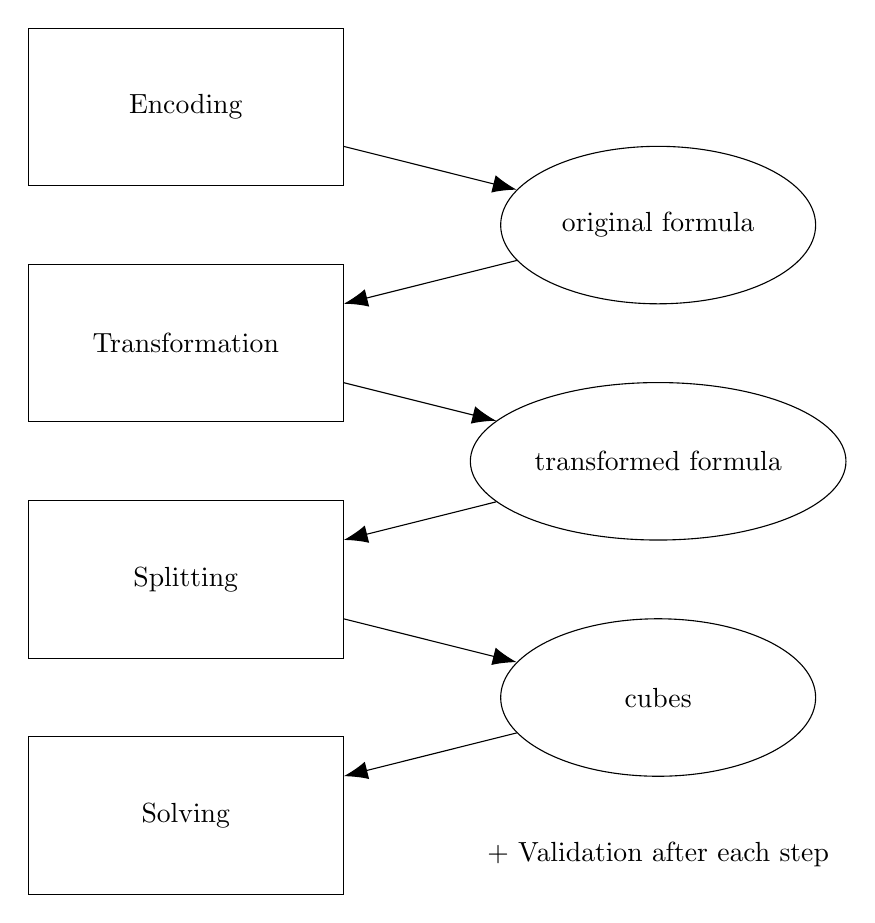
\begin{tikzpicture}[x=1cm,y=1cm]

\node (e1) at (6,7.5) [draw,ellipse,minimum width=4cm,minimum height=2cm] {original formula};
\node (e2) at (6,4.5) [draw,ellipse,minimum width=4cm,minimum height=2cm] {transformed formula};
\node (e3) at (6,1.5) [draw,ellipse,minimum width=4cm,minimum height=2cm] {cubes};

\node (r1) at (0,9) [draw,rectangle,minimum width=4cm,minimum height=2cm] {Encoding};
\node (r2) at (0,6) [draw,rectangle,minimum width=4cm,minimum height=2cm] {Transformation};
\node (r3) at (0,3) [draw,rectangle,minimum width=4cm,minimum height=2cm] {Splitting};
\node (r4) at (0,0) [draw,rectangle,minimum width=4cm,minimum height=2cm] {Solving};

\draw [-{Latex[scale=1.8]}] (r1) edge (e1) (e1) edge (r2) (r2) edge (e2) (e2) edge (r3) (r3) edge (e3) (e3) edge (r4);

\node at (6,-0.5) {+ Validation after each step};

\end{tikzpicture}
\end{document}